\documentclass[twocolumn, 12pt]{report}
\usepackage{graphicx}

\renewcommand*\thesection{\arabic{section}}




% Title Page
\title{Effects of Fish Consumption on the Level of Mercury in the Hair of Fishermen}
\author{Haylem Rayner}


\begin{document}

\bibliographystyle{ieeetr}
\maketitle

\begin{abstract}
	Methyl-Mercury Concentrations are analysed as they're the most common form of Mercury ingestion. The consumption of fish is measured by the average number of fish meals consumed per week. The results show that there is no significant relationship between the number of meals consumed per week among fishermen and their MeHg concentrations.
\end{abstract}


\section{Introduction}

It is widely recognized that mercury can be toxic to humans in any form \cite{kim2016review}. Methyl-Mercury is a particular organic form of elemental mercury present in fish. It is the most common form of mercury ingested by humans. I will perform regression analysis on the number of fish meals consumed per week to assess the relationship toward MeHg concentrations in Kuwait Fishermen.



\section{Materials and Methods}

The data set provided is a survey of Total and Methyl-Mercury from fishermen in the village of Doha, Kuwait. 100 samples of hair were collected to measure the mercury concentrations, each taken from several sites of the scalp until a total mass of 2-3 g was achieved. These mercury samples were then processed according to a standard set of procedures described by \cite{al2000factors}. Each fishermen was then asked to complete a questionnaire to record their age, nationality, occupation, duration of stay in Kuwait, smoking habits, health status (particularly regarding any amalgam fillings which would effect mercury levels) and their dietary habits. 


\section{Results}

The total and Methyl-Mercury measurements are highly correlated. This is to be expected since MeHg is the most common form of organic mercury transferred to humans, particularly via consumption of fish. For this reason the analysis will focus on investigating the relationship between consumption of fish and MeHg.

There is a moderately positive correlation between meals of fish per week and MeHg as seen in figure \ref{fig:all}. The only response of meals per week from fishermen were for 3, 4, 7, 14 and 21. Those eating less than seven meals per week of fish made up 14\% of the entire dataset, 16\% ate more than seven with the remaining 70\% recording that they eat exactly seven meals per week of fish. This would indicate that most fishermen are having a single meal of fish per day, per week. As there are few examples of fishermen having less than or greater than seven meals per week the response variable was categorized into; less than seven meals per week, seven meals per week and greater than seven meals per week. This loosely corresponds to `eating fish less than once a day', `eating fish each day' and `eating fish more than once a day'.

Within the smallest and largest consumption groups there appear to be some outliers, noticeable in figure \ref{fig:all}. There doesn't appear to be any correlation between these outliers and so initial analysis will include all data points.

\begin{figure}
	\begin{tabular}{c}
		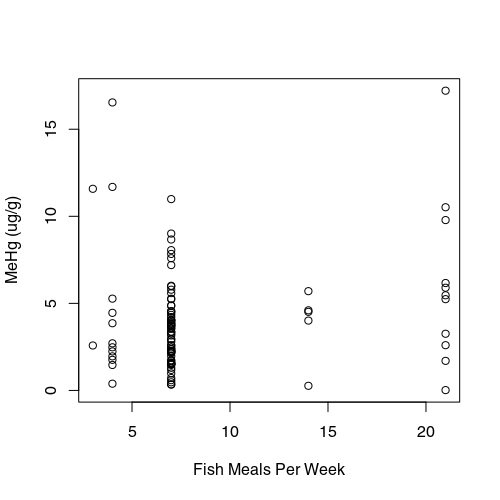
\includegraphics[width=\linewidth]{res/all.png} \\
		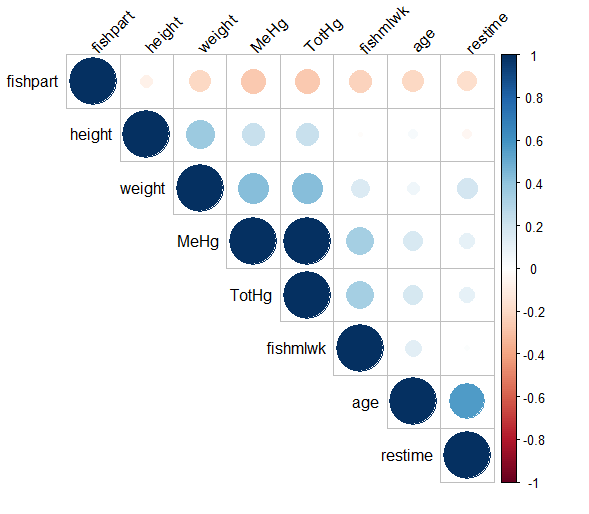
\includegraphics[width=\linewidth]{res/correlation.png}
	\end{tabular}
	\caption{Total data set (top) and correlation between all variables (bottom)} 
	\label{fig:all}
\end{figure}

\subsection{Weight}

There is a moderately strong correlation between MeHg and body weight as seen in figure \ref{fig:all}. It seems likely there would be some effect of percentage body fat on the metabolism which could then lead to decreasing the burden of MeHg in the body. In this dataset information exists only for the total weight, so this effect cannot be investigated. Figure \ref{fig:all} shows a moderately positive correlation between weight and both MeHg and Total Mercury concentrations. This could be due to weight being correlated with increased consumption of the actual \emph{amount} of fish during any one sitting.  

\subsection{Fish Part}

There is a moderately strong negative correlation between Meal per week of fish and preferred part of fish to consume. Of all fishermen 19\% preferred to consume the muscle only, 72\% preferred the muscle and sometimes the whole fish with the remaining 9\% preferring both.

\begin{figure}
	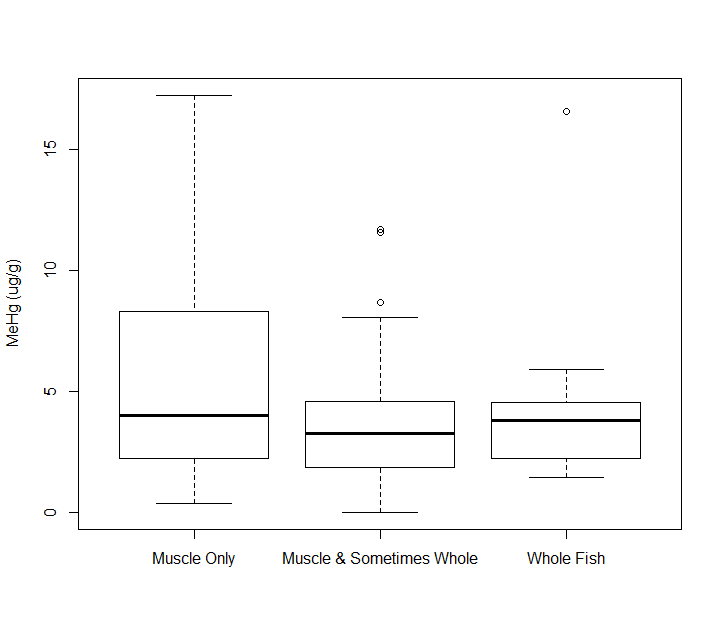
\includegraphics[width=\linewidth]{res/me_fishpart.png}
	\caption{Preferred fish part for consumption}
	\label{fig:fishpart}
\end{figure}

\subsection{Meals Consumed per week}

Across all data points and within groups based on fish consumption per week the MeHg concentration is right skewed. This is to be expected with the MeHg being non-negative and small in magnitude. For this reason general linear modelling was performed using a Gamma distribution. Backward step-wise AIC selection was employed to select the optimal model which was found to be:

\[MeHG = Height + Weight + Meals\]

T-tests showed height as significant to a 10\% critical value, weight significant to 1\% and seven fish meals per week significant to 10\%. The resulting regression coefficients indicate a unit increase in height multiplicatively effecting the expected MeHg concentration within a range of 0.85 and 1.22, weight effecting MeHg concentration within a range of 0.86 and 1.25 and seven meals per week effecting MeHg concentration within a range of 0.32 and 1.69.

\begin{figure}
	\begin{tabular}{c}
		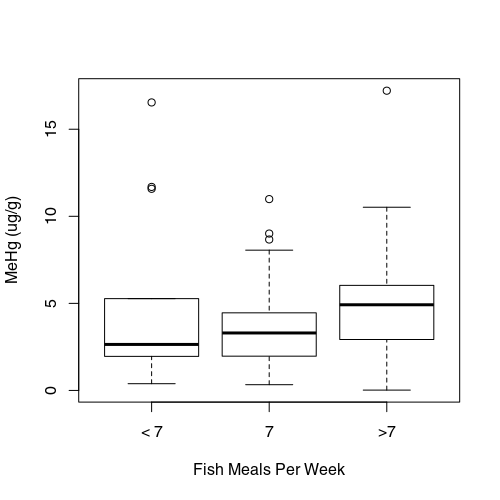
\includegraphics[width=\linewidth]{res/me_meals_dirty.png} \\
		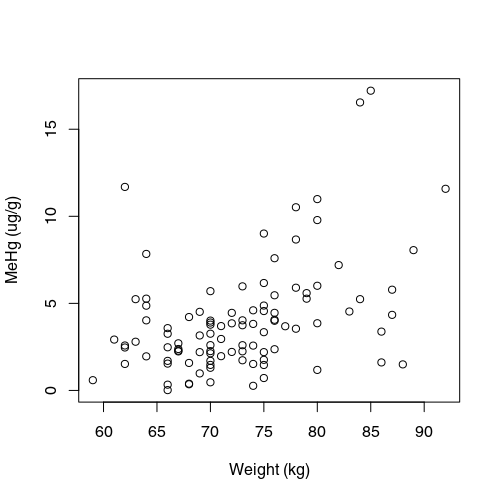
\includegraphics[width=\linewidth]{res/me_weight_dirty.png}
	\end{tabular}
	\caption{Methyl-mercury with outliers present}
	\label{fig:methyl dirty}
\end{figure}

\subsection{Control Results}

Identical data was collected across 30 control subjects, who were not fishermen. As seen in figure \ref{fig:control} there is a much more even distribution of fish meals consumed per week among the control group. For this reason when performing the same regression procedure as for the fishermen the variable for meals consumed per week was not categorized. When doing so the optimal model according to backward step-wise AIC selection is:

\[MeHg = Meals\]

T-tests showed meals as significant to a 1\% critical value. The resulting regression coefficient indicates a unit increase in meals consumed per week multiplicatively effects the expected MeHg concentration within a range of 1.42 and 3.25. 

\begin{figure}
	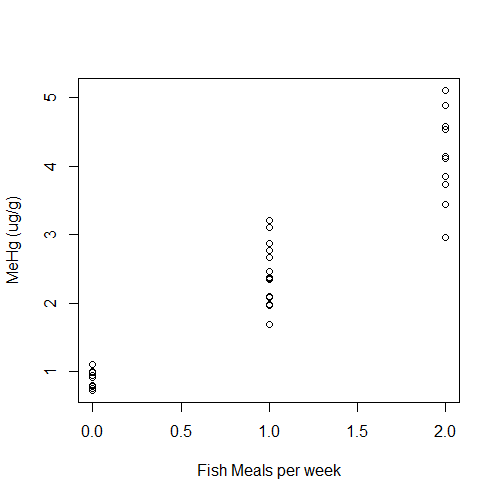
\includegraphics[width=\linewidth]{res/control_meals.png}
	\caption{Concentration of Methyl-Mercury among control group}
	\label{fig:control}
\end{figure}
   
\section{Discussion}

\subsection{Measurement of Fish Consumed}

Assessment of the amount of fish consumed by an individual was done by requesting the average number of fish meals consumed pre week. Most fishermen would be expected to consume a large amount of fish, which is evident in the large proportion that consume on average one fish meal per day. It is very unlikely to reflect the actual quantity of fish product  consumed. Simple dietary difference such as eating a single meal per day would effect the serving size of any number of meals per day. This could explain those outliers at less than seven fish meals per week, those individuals may be consuming a large \emph{quantity} of fish at any one time. An individual who responds with 21 meals per week could have 3 meals of fish each day while still only consuming the same amount of fish as an individual having a single meal of fish per day but 3 times the portion size.

\subsection{Diversity of Fish Available}

It has been well established that Methyl-Mercury levels vary substantially among different fish species \cite{al-Majed2000}. Although the fishermen stated they have `no preference for type of fish' \cite{al2000factors} it`s possible there are difference in the species consumed. Factors such as availability of fish in different catchments zone could result in fishermen consuming fish with varying levels of MeHg.  

\subsection{Control Group}

The meals of fish per week is much more significant among the control group. There is a stronge correlation toward MeHg which could indicate that there are less latent effects `masked' by this meal per week variable. At this smaller number of meals consumed per week the response is likely to be more salient. When an individual responds with zero meals of fish per week this would indicate they rarely, if ever consume fish. Then either one or two meals per week would be a marked increase in fish consumption.

\section{Conclusion}

There does not appear to be a clear relationship between the number of fish meals consumed per week and the levels of either MeHg or Total mercury among the fishermen in Kuwait. After categorizing fishermen into three distinct `consumption' levels there is no significant effect on MeHg as the meals consumed per week increases. This is likely due to latent variables such as the quantity of fish consumed at each sitting and variety of MeHg concentration among different fish species. The average `meals per week' response is not a well defined measure of the actual consumption of fish. Constructing a more quantitative measure of fish consumption could indicate the effect on MeHg more clearly.   

\bibliography{sources}
\end{document}    

   
